\documentclass[12pt]{article}

%packages
\usepackage[ngerman]{babel}
\usepackage[a4paper, total={7in, 10.2in}]{geometry}
\usepackage{enumitem}
\usepackage{tabularx}
\usepackage{makecell}
\usepackage{graphicx}

%general definitions
\pagestyle{empty}
\setlist{noitemsep}
{\renewcommand{\arraystretch}{1.5}%

\begin{document}
	\begin{minipage}[b]{13cm}
		\section*{Persönliche Daten}
		\begin{tabularx}{\textwidth}{b{4cm}|l}
			Name & Benedikt Schmidt \\
			Adresse & Pradler Straße 69, Innsbruck, Österreich \\
			Geburtsdatum & 26. September 1990 \\
			Kontaktdaten & +4366488742636, benediktibk@gmail.com \\
			Homepage & http://me.benediktschmidt.at
		\end{tabularx}		

		\section*{Berufserfahrungen}
		\begin{tabularx}{\textwidth}{b{4cm}|b{3cm}|l}
			\thead{von} & \thead{bis} & \\
			Oktober 2017 & heute & Leading Operations Engineer bei world-direct \\
			Juni 2016 & November 2017 & \makecell[cl]{Selbstständiges Gewerbe für Dienstleistungen \\ in der Informationstechnik} \\
			April 2015 & September 2017 & Development/Operations VoIP bei world-direct \\
			Juli 2012 & März 2015 & \makecell[cl]{Studentische Hilfskraft am Sprachenzentrum der \\ Technischen Universität München} \\
			September 2011 & September 2011 & Junior Software Developer bei Datacon \\
			Jänner 2011 & April 2011 & Junior Software Developer bei Datacon \\
			Juli 2008 & Juli 2008 & \makecell[cl]{Innovationspraktikant am Institut für Mathematik \\ der Universität Innsbruck}
		\end{tabularx}
		
		\section*{Ausbildung}
		\begin{tabularx}{\textwidth}{b{4cm}|b{3cm}|l}
			\thead{von} & \thead{bis} & \\
			Februar 2016 & November 2016 & CCNP Collaboration \\
			Oktober 2013 & März 2015 & \makecell[cl]{Master Elektro- und Informationstechnik an der \\ Technischen Universität München} \\
			Mai 2011 & Oktober 2013 & \makecell[cl]{Bachelor Elektro- und Informationstechnik an der \\ Technischen Universität München} \\
			September 2005 & Juni 2010 & HTL Elektrotechnik Anichstraße, Innsbruck
		\end{tabularx}
		
		\section*{Kompetenzen}
		\begin{tabularx}{\textwidth}{b{4cm}|l}
			Programmiersprachen & \makecell[cl]{C\#, C/C++, Python, VHDL, Javascript, Bash, Matlab, \\ Powershell, SQL} \\
			Webdesign & HTML, CSS \\
			Netzwerk & \makecell[cl]{CCNP Collaboration, fundierte Kenntnise von diversen Protokollen \\ (IP, TCP/UDP, Ethernet, HTTP, SIP, RTP, ...)} \\
			Versionskontrolle & git, mercurial, Subversion \\
			Anwendungen & Visual Studio, Wireshark, IIS, nginx, iptables, Zabbix, MS SQL, ... \\
			Betriebssysteme & Windows, Linux
		\end{tabularx}
	\end{minipage}	
	\begin{minipage}[t]{3cm}
		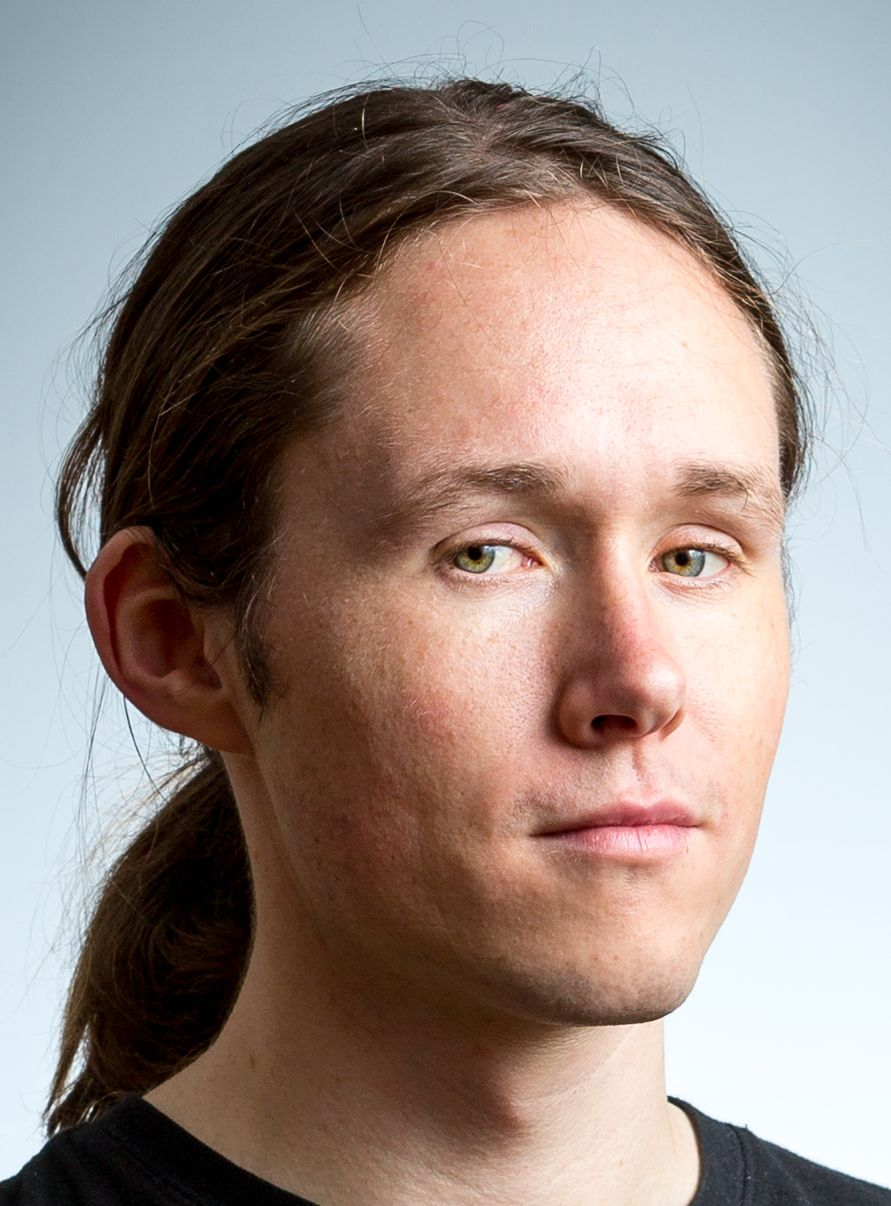
\includegraphics[width=3cm]{portrait.jpg}
	\end{minipage}
\end{document}